Joana já regressou para dentro de sua casa. Brincou o dia inteiro na natureza e com ela.
Agora o sol está próximo do horizonte, quase a despedir-se do jardim.

\textbf{Eu sou Eu} observa os pequenos insetos ainda em estado de êxtase e empapados em Amor.

E neste momento de Paz começa a entoar um poema, escrito por uma criança como a menina do jardim.

E mesmo os insetos mais distraídos, absorvem o fluxo silencioso de Energia que aquelas palavras difundem.
\bigbreak
Poema:
\bigbreak
“Pergunta ao teu Coração”

“O que fará o Amanhecer um momento tão belo e mágico,

Que só ele é capaz de marcar um novo dia,

Um recomeço com tal esplendor,

Que nos permite, a nós que o contemplamos verdadeiramente,

Ter o ânimo para repetir aquele perpétuo ciclo
Que nos diz tão pouco, o nosso dia a dia,

Quase parecendo que o único motivo pelo qual o toleramos

Por tão longas horas de espera descrente,

É o insaciável desejo, inexplicável por palavras,

De voltar a ver o Sol cruzar o horizonte?
\bigbreak
Será apenas a quietude da sua beleza bizarra,

Aquela fusão de tudo o que faz magnífica a simples existência,

Mas da mais genuína Essência, que mesmo sem exigências ou expectativas

Consegue tornar-se no Todo,

Cuja ausência tiraria o sentido ao Nada que restasse?
\bigbreak
É a sua criação que torna o Criador tão admirável e incontestável

Não só o Criador em si, já que depende da criação para existir,

E da mesma forma, a obra precisa do artista para nascer.

Afinal, é tudo um perfeito ciclo.
\bigbreak
É a vida que o Sol ilumina que nos faz sentir tanta saudade ao recolher,

O pôr do sol, o seu polo gelado, a despedida com que nos saúda

Eternamente imperturbável.

E apesar de certo que voltará no novo Amanhecer,
Continuamos a chorá-lo com nostalgia e temor,
Porque perdendo o Sol, perdemos tudo.
\bigbreak
GIRAMOS TODOS À VOLTA DO MESMO AMOR!”
\bigbreak
Os insetos batem palmas, ou melhor, batem as patas quando terminam de escutar aquele poema tão belo que descreve a força e a magia do astro-Rei no nosso pequeno planeta.
\bigbreak
O Sol começa a esconder-se atrás das árvores guardiãs. \textbf{Eu sou Eu} tem de partir.
\bigbreak
Então, faz-se um silêncio no jardim, os olhinhos da bicharada estão brilhantes, com lágrimas.

O AnThaisiano diz-lhes:
\bigbreak
\begin{figure}[h]
    \centering
    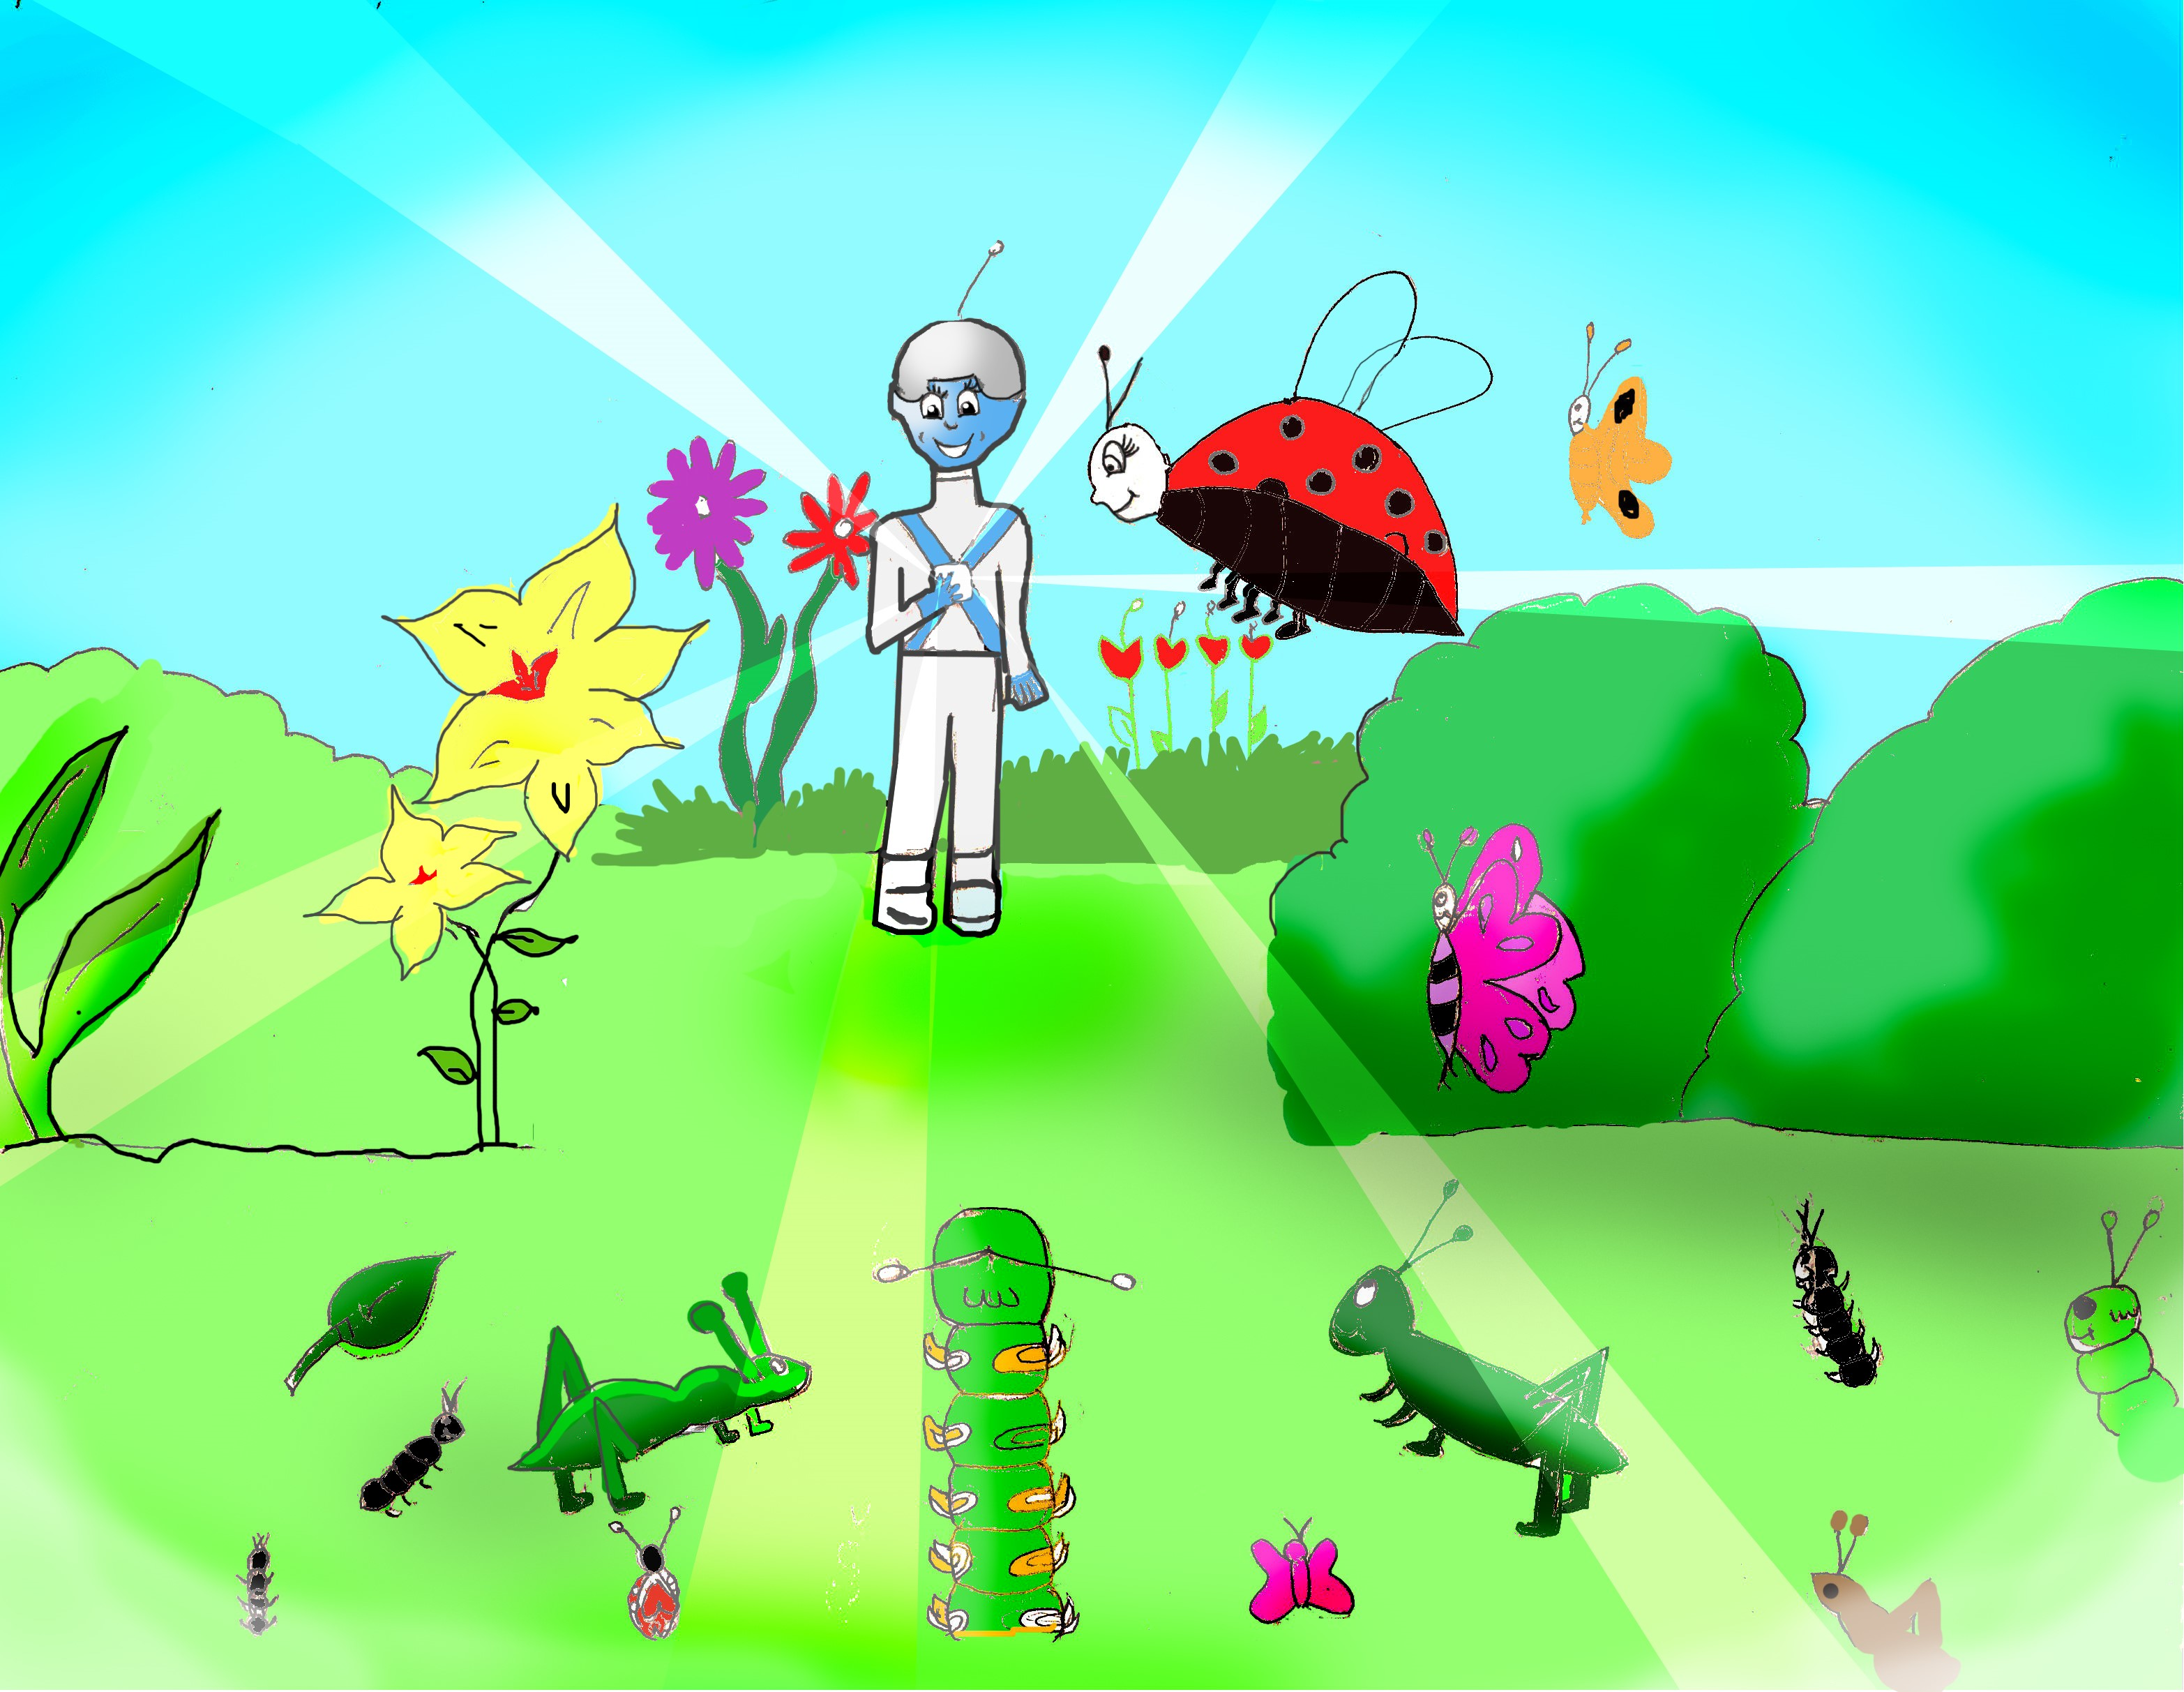
\includegraphics[width=0.85\textwidth]{ultima}
\end{figure}

— Levo-vos dentro do meu coração. E fico aqui, dentro do vosso. Sempre que fecharem os olhos e focarem no centro dele, eu estou lá e converso com cada um. Agora tenho de ir. Até sempre e mais Além.
\bigbreak
\textbf{Eu sou Eu} com a mão esquerda regula a antena interplanetária do seu capacete e entra em comunicação com o seu planeta – AnThais. Do nada surge um feixe luminoso que o envolve e se transforma numa Esfera Transdimensional.

O vento que o observa, exala uma brisa perfumada e a ET eleva-se no ar, como uma bola de sabão, sem peso e transparente, desaparecendo no céu.

Os insetos recolhem-se nas suas tocas porque o sol já se despediu, deixando no jardim uma temperatura amena, porque hoje... começou a Primavera.
